\section{Incidence Extensions: Local versus National Policy}\label{sec:decentralized}

Section \ref{sec:subsidy} derived a primitive benchmark in which optimal subsidies and comparative statics are determined entirely by product-market primitives together with the endogenous merger-attempt condition. This section reintroduces planner-specific local retention and spillover incidence as adjustments around that benchmark. The comparison is not a strategic game across jurisdictions. For a fixed project type, the local--national difference is an incidence comparison around the primitive benchmark. What buyout exit adds is that the privately selected project can switch with merger permissiveness, thereby changing the relevant incidence comparison itself.

\subsection{Planner-specific incidence adjustments around the primitive benchmark}

Let $B_j^p(q)$ denote planner-$p$ successful-project value, and define the planner-specific incidence adjustment relative to the primitive benchmark by
\begin{equation}\label{eq:Djp}
    D_j^p(q)\equiv B_j^p(q)-B_j^{PM}(q).
\end{equation}
Planner-$p$ welfare conditional on project $j$ is
\begin{equation}\label{eq:Wjp}
    W_j^p(s,q)
    =
    \int_0^{c_j(s,q)}
    \left[
        R_j(q)B_j^p(q)-\frac{R_j(q)^2}{2}-f-\tau s
    \right]df,
\end{equation}
where the private entry cutoff remains
\begin{equation}
    c_j(s,q)=s+\frac{R_j(q)^2}{2}.
\end{equation}

\begin{proposition}\label{prop:incidencedecomp}
Fix a project type $j$ and an approval probability $q$. Let
\begin{equation}\label{eq:uPM}
    u_j^{PM}(q)
    \equiv
    \frac{
        R_j(q)B_j^{PM}(q)-\frac{\tau+2}{2}R_j(q)^2
    }{2\tau+1}.
\end{equation}
Then the planner-$p$ optimal subsidy is
\begin{equation}\label{eq:incidencedecomp}
    s_j^{p*}(q)
    =
    \max\left\{
        0,\;
        u_j^{PM}(q)+\frac{R_j(q)D_j^p(q)}{2\tau+1}
    \right\}.
\end{equation}
If, in addition, both the primitive benchmark subsidy and the planner-$p$ subsidy are interior at $(j,q)$, then
\begin{equation}\label{eq:incidencedecompinterior}
    s_j^{p*}(q)
    =
    s_j^{PM*}(q)
    +
    \frac{R_j(q)D_j^p(q)}{2\tau+1}.
\end{equation}
\end{proposition}

Proof is reported in Appendix \ref{app:decentralized}.

Proposition \ref{prop:incidencedecomp} places planner-specific incidence adjustments around the primitive benchmark in a way that remains valid globally once corner solutions are respected. The exact additive decomposition uses $s_j^{PM*}(q)$ only on interior regions where the primitive benchmark itself is not at the subsidy corner.

\subsection{Local and national planners as special cases}

For the local planner, let
\begin{align}
    B_j^{L,D}
    &\equiv
    C^D(j)
    + \lambda_I^L \pi_I^D(j)
    + \lambda_E^L \pi_E^D(j)
    + \eta_j^D, \label{eq:BLD} \\
    B_j^{L,A}
    &\equiv
    C^M(j)
    + \lambda_M^L \Pi^M(j)
    + \eta_j^A. \label{eq:BLA}
\end{align}
With local attempt-cost share $\kappa^L\in[0,1]$, successful-project value is
\begin{equation}\label{eq:BLq}
    B_j^L(q)
    =
    B_j^{L,D}
    +
    a_j(q)
    \left[
        q\bigl(B_j^{L,A}-B_j^{L,D}\bigr)-\kappa^L k
    \right].
\end{equation}
Appendix \ref{app:subsidy} develops useful decompositions for the local incidence block, including retained buyout proceeds and local spillover losses.

For the national planner, let
\begin{align}
    B_j^{N,D}
    &\equiv
    C^D(j)+\pi_I^D(j)+\pi_E^D(j)+\xi_j^D, \label{eq:BND} \\
    B_j^{N,A}
    &\equiv
    C^M(j)+\Pi^M(j)+\xi_j^A. \label{eq:BNA}
\end{align}
With national attempt-cost share $\kappa^N\in[0,1]$, successful-project value is
\begin{equation}\label{eq:BNq}
    B_j^N(q)
    =
    B_j^{N,D}
    +
    a_j(q)
    \left[
        q\bigl(B_j^{N,A}-B_j^{N,D}\bigr)-\kappa^N k
    \right].
\end{equation}
As special cases of \eqref{eq:Djp}, the local and national incidence adjustments are
\begin{equation}
    D_j^L(q)=B_j^L(q)-B_j^{PM}(q),
    \qquad
    D_j^N(q)=B_j^N(q)-B_j^{PM}(q).
\end{equation}

\begin{corollary}\label{cor:wedgefixed}
If both local and national optimal subsidies are interior, then for any fixed project type $j$,
\begin{equation}\label{eq:wedgefixed}
    s_j^{L*}(q)-s_j^{N*}(q)
    =
    \frac{R_j(q)\bigl(B_j^L(q)-B_j^N(q)\bigr)}{2\tau+1}.
\end{equation}
Hence the sign of the fixed-project wedge is the sign of $B_j^L(q)-B_j^N(q)$.
\end{corollary}

Proof is reported in Appendix \ref{app:decentralized}.

Corollary \ref{cor:wedgefixed} shows that once the primitive benchmark has been isolated, the fixed-project local--national wedge is an algebraic incidence comparison. Appendices \ref{app:sufficientlocalover} and \ref{app:sufficientlocalunder} give sufficient conditions for positive and negative wedges in terms of retained buyout proceeds and locally concentrated post-acquisition losses.

\subsection{Equilibrium wedges under private project choice}

Reintroduce private project choice. Let
\begin{equation}
    j^*(q)\in\{I,B\}
\end{equation}
denote the entrepreneur's privately optimal project and define
\begin{equation}
    \bar R(q)\equiv R_{j^*(q)}(q),
    \qquad
    \bar B^L(q)\equiv B_{j^*(q)}^L(q),
    \qquad
    \bar B^N(q)\equiv B_{j^*(q)}^N(q).
\end{equation}

\begin{corollary}\label{cor:wedgeequilibrium}
Suppose Assumptions \ref{ass:types}--\ref{ass:singlecross} hold and both planner-specific subsidies are interior on the relevant range. Then
\begin{equation}\label{eq:wedgeequilibrium}
    s^{L*}(q)-s^{N*}(q)
    =
    \frac{\bar R(q)\bigl(\bar B^L(q)-\bar B^N(q)\bigr)}{2\tau+1}.
\end{equation}
In particular, if
\begin{equation}
    B_I^L(q)<B_I^N(q)
    \quad\text{for } q<\hat q,
    \qquad\text{and}\qquad
    B_B^L(q)>B_B^N(q)
    \quad\text{for } q>\hat q,
\end{equation}
then the sign of the equilibrium subsidy wedge changes at the project-switching threshold.
\end{corollary}

Proof is reported in Appendix \ref{app:decentralized}.

For illustration, Figures \ref{fig:local_national_subsidies_calibrated}--\ref{fig:wedge_calibrated}
use the following parameterization:
\[
a_I=1.2,\quad \sigma_I=0.5,\quad m_I=0.05,
\qquad
a_B=1.1,\quad \sigma_B=0.3,\quad m_B=0.15,
\]
\[
\beta=0.35,\quad k=0.03,\quad \tau=1,
\]
together with
\[
\lambda_I^L=0.2,\quad \lambda_E^L=0.7,\quad \lambda_M^L=0.15,
\]
\[
\eta_I^D=0.10,\quad \eta_I^A=0.05,\quad \eta_B^D=0.08,\quad \eta_B^A=0.02,
\]
\[
\xi_I^D=0.12,\quad \xi_I^A=0.08,\quad \xi_B^D=0.10,\quad \xi_B^A=0.04,
\qquad
\kappa^L=\kappa^N=1.
\]
These values imply
\[
\bar q_B \approx 0.1908,\qquad
\bar q_I \approx 0.4461,\qquad
\hat q \approx 0.6531.
\]
The calibration is chosen only to illustrate the qualitative comparative statics and threshold ordering of the model; it is not intended as a quantitative fit to any specific institutional setting.

\begin{figure}[t]
\centering
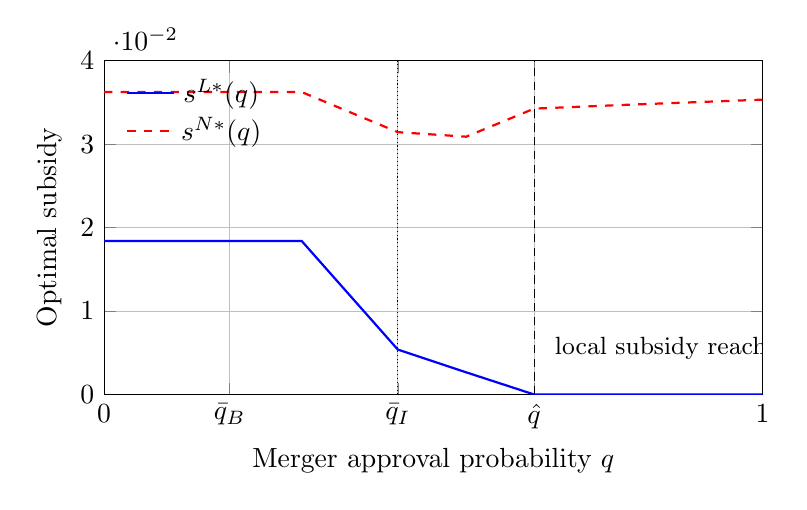
\begin{tikzpicture}
\begin{axis}[
    width=0.82\textwidth,
    height=0.48\textwidth,
    xmin=0, xmax=1,
    ymin=0, ymax=0.04,
    xlabel={Merger approval probability \(q\)},
    ylabel={Optimal subsidy},
    legend style={draw=none, fill=none, at={(0.02,0.98)}, anchor=north west},
    xtick={0,0.1907549041,0.4461335096,0.6531405543,1},
    xticklabels={0,\(\bar q_B\),\(\bar q_I\),\(\hat q\),1},
    ymajorgrids=true,
    xmajorgrids=true
]

\addplot[thick, blue] coordinates {
(0,0.01840865870)
(0.1,0.01840865870)
(0.1907549041,0.01840865870)
(0.3,0.01840865870)
(0.4461335096,0.00538027289)
(0.55,0.00265601444)
(0.6531405543,0)
(0.8,0)
(1,0)
};
\addlegendentry{\(s^{L*}(q)\)}

\addplot[thick, red, dashed] coordinates {
(0,0.03625141202)
(0.1,0.03625141202)
(0.1907549041,0.03625141202)
(0.3,0.03625141202)
(0.4461335096,0.03144295670)
(0.55,0.03089882779)
(0.6531405543,0.03426378692)
(0.8,0.03474278419)
(1,0.03533919386)
};
\addlegendentry{\(s^{N*}(q)\)}

\addplot[densely dotted, black] coordinates {(0.4461335096,0) (0.4461335096,0.04)};
\addplot[densely dashed, black] coordinates {(0.6531405543,0) (0.6531405543,0.04)};

\node[anchor=south west] at (axis cs:0.67,0.003) {\small local subsidy reaches zero};
\end{axis}
\end{tikzpicture}
\caption{Illustrative local and national optimal subsidies under the calibration reported in the text. The figure plots the constrained planner-specific optima, including the subsidy corner at zero. Accordingly, the interior closed-form expressions that underlie Corollaries \ref{cor:wedgefixed} and \ref{cor:wedgeequilibrium} apply only on subregions where the relevant planner-specific subsidies remain strictly positive. In this calibration, easier buyout exit weakens the case for local subsidy, and the local planner withdraws support after the switch to buyout-oriented entrepreneurship.}
\label{fig:local_national_subsidies_calibrated}
\end{figure}

\begin{figure}[t]
\centering
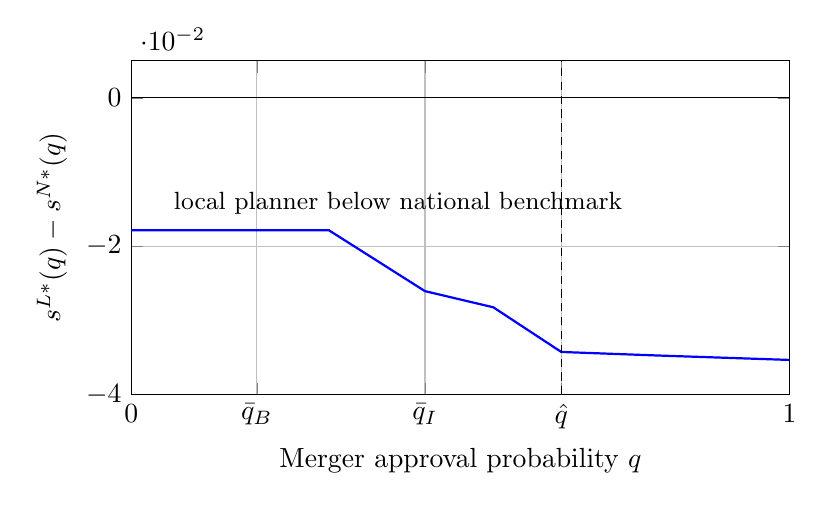
\begin{tikzpicture}
\begin{axis}[
    width=0.82\textwidth,
    height=0.48\textwidth,
    xmin=0, xmax=1,
    ymin=-0.04, ymax=0.005,
    xlabel={Merger approval probability \(q\)},
    ylabel={\(s^{L*}(q)-s^{N*}(q)\)},
    xtick={0,0.1907549041,0.4461335096,0.6531405543,1},
    xticklabels={0,\(\bar q_B\),\(\bar q_I\),\(\hat q\),1},
    ymajorgrids=true,
    xmajorgrids=true
]

\addplot[thick, blue] coordinates {
(0,-0.01784275331)
(0.1,-0.01784275331)
(0.1907549041,-0.01784275331)
(0.3,-0.01784275331)
(0.4461335096,-0.02606268381)
(0.55,-0.02824281335)
(0.6531405543,-0.03426378692)
(0.8,-0.03474278419)
(1,-0.03533919386)
};
\addplot[thin, black] coordinates {(0,0) (1,0)};
\addplot[densely dashed, black] coordinates {(0.6531405543,-0.04) (0.6531405543,0.005)};

\node[anchor=south west] at (axis cs:0.05,-0.017) {\small local planner below national benchmark};
\end{axis}
\end{tikzpicture}
\caption{Illustrative local--national incidence wedge around the primitive benchmark under the calibration reported in the text. The plotted wedge is the difference between the constrained optimal subsidies from Figure \ref{fig:local_national_subsidies_calibrated}. Hence, once one planner hits the zero-subsidy corner, the plotted wedge need not coincide with the interior formula in Corollary \ref{cor:wedgeequilibrium}. In this benchmark-consistent calibration, the local planner values successful entrepreneurial entry less than the national planner throughout, so the wedge remains negative even though its magnitude changes discretely when project choice switches.}
\label{fig:wedge_calibrated}
\end{figure}

\subsection{Discussion}

Section \ref{sec:subsidy} established that the main subsidy comparative statics are first pinned down by the primitive benchmark objects $\Delta_j$ and $\Omega_j$. The local and national results here are planner-specific adjustments around that benchmark.

This ordering clarifies the interpretation of the wedge results. For a fixed project, the sign of the local--national difference is an incidence comparison. What buyout exit adds is that merger permissiveness can change the privately selected project, thereby changing the economically relevant incidence comparison. Appendix Figure \ref{fig:wedge_sign_reversal_appendix} reports a transfer-augmented calibration illustrating the sign-reversal case highlighted in Corollary \ref{cor:wedgeequilibrium}.
